\chapter{Introduction}

Standard computer systems are hierarchically organized in a three
layers stack, as depicted in figure \ref{fig:3ls}. The lowest layer is the bare hardware, the middle one is the operating system and the 
upper layer contains the applications software.
Two neighbor layers can communicate through a well-defined \emph{interface}, so that each layer can ignore how the
lower layers are actually implemented. In this way, the interface provides an \emph{abstraction} of the underlying software/hardware
resources.

\begin{figure}[bt]
\centering
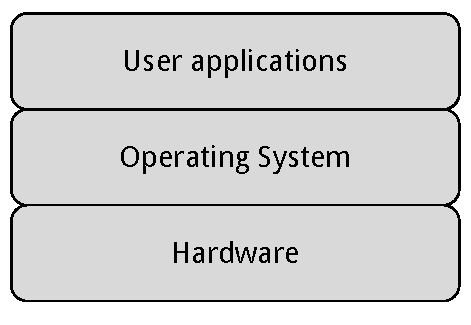
\includegraphics[scale = 1.0]{3-layers-stack.pdf}
\caption{A standard 3-layers-stack computer system}
\label{fig:3ls}
\end{figure}

This (relatively) simple architecture has proven to be very effective in delivering the IT services required
by companies, individual users and other organizations.

\vspace{0.5cm}

Neverthless, more complex computer systems organizations have been devised and used, in order to overcome some limitations
of the standard computer system model.

These computing environments are are known as \emph{Virtual Machines} (VMs) systems.
By itself, the term \emph{Virtual Machine} can have several meanings, so when using it is important to point out what we are
addressing. In section \ref{sec:vmclass} we will provide a classification of these meanings.
In general \emph{virtualization} provides a way of increasing the \emph{flexibility} of real hardware/software resources. When a 
physical resource is virtualized, it can appear to be a resource of a different kind or even a \emph{set} of different
resources (the same kind or different kind).

As an example, a single IA32 processor can be virtualized in a way that emulates more PowerPC processors. Once this is done, you
can build many standard 3-layer computer systems on top of each emulated PowerPC (virtual) processor, using unmodified OS and 
applications designed to be used on the PowerPC architecture.

\vspace{0.5cm}

We talk about Virtual Machines when we virtualize a physical computing enviroment (e.g a server machine) and get one or more 
independent virtual computing environment (the VMs), potentially different by the original one.

In the VMs terminology, each VM is also called \emph{guest}, whereas the virtualized physical computing environment is known as
\emph{host}.
The piece of software that provides the support for virtualization is called \emph{Virtual Machine Monitor} (VMM) or \emph{Hypervisor}.

You can virtualize nearly all the resources you wants: disks, network devices, memories or other peripherals.

\vspace{0.5cm}

Generally speaking VMs allow to build computer systems with more abstraction levels than the standard model has. This has important
advantages:
\begin{itemize}
  \item In terms of \emph{flexibility}, using VMs you can easily run programs compiled for a given Instruction Set Architecture (ISA) 
	and a given Operating System (OS) on top of a computer system that has a different ISA and/or a different OS. Using a standard
	system you would be bound to the ISA of your processor and the operating system installed on your machine. This flexibility can be 
	exploited in several situations, such as testing new software on different architectures (without physically have the
	machines supporting each different architecture), or run legacy applications on newer, more power-efficient hardware.

  \item In terms of \emph{protection}, VMs can provide multiple isolated execution environments running on the same phisical machine.
	This allows to execute different applications in different VMs (each VM can have its own OS), so that if an application has a
	security hole, an attacker cannot use the hole to do malicious attacks to an applications running on a different VM. 
	This scenary is still possible when applications are run in the same OS.
	
  \item In terms of resources usage, VMs can help to reduce hardware costs and power consumption, since they naturally improve 
	resource utiliziation. For instance, you can use only one physical server machine to provide multiple services (without 
	sacrifying isolation), using the 100\% of the machine resource, instead of using many underutilized server machines
	\footnote{Assuming, as often happens, that one or a few services don't utilize all the computing resource offered by
	a modern server machine.}. This results in money and energy saving.
	
  \item In terms of \emph{mobility}, you can easily migrate VMs (and so replicate them) to other locations, simply transmitting 
	some files through the Internet. This can also help avoiding setup times (software installation and configuration), 
	since through a VM you can convey a ready-to-use copy of a computing environment to the user.
\end{itemize}

The previous list is not exhaustive, but gives an idea of the services that virtualization can deliver, and makes clear the reasons
why IT departments make massive use of virtualization technologies.



\section{Virtual Machines classification}
\label{sec:vmclass}

As noted previously, the term \emph{Virtual Machine} can have several meanings. Therefore it is useful to give
a classification of the possible meanings (see \cite{ref:vmclassification} section 1.5 in \cite{ref:vmbook}).

First of all, VM can be divided in two categories:
\begin{itemize}
    \item \emph{System Virtual Machines}: these VMs provides virtualization at ISA level. This means that the VM is capable of executing 
	  arbitrary code compiled for a specified ISA.  System virtual machines provides a complete executing environment where
	  multiple processes can be run.
	  A system VM can then be used to run an OS that supports several applications, namely a standard 3-layers computer
	  environment.
	  
    \item \emph{Process Virtual Machines}: these VMs virtualize at the Application Binary Interface (ABI) level, providing
	  an execution environment for a single application. Since
	  applications are usually written in high level languages and so use an high level interface\footnote{For instance an OS 
	  system call interface, or the interface provided by an interpreted programming language.}, if we want to execute a single
	  application, the VM is only required to emulate the high level interface and/or a subset of the ISA\footnote{Typically 
	  unprevileged instructions, and instructions that are not problematic with respect to CPU virtualization (see \cite{ref:x86-virt}
	  and section 8.2 in \cite{ref:vmbook}).}. User applications are therefore provided with a virtual ABI anvironment.
\end{itemize}

\subsection{System level Virtual Machines}
System virtual machines can be further divided depending on whether the code executed in the VM (the guest) is of the same ISA
of the physical machine supporting the VM (host).

The same-ISA case is very common, since users are often interested in server consolidation (resource usage optimization), protection or
live migration, but don't care about executing code compiled for a specific ISA. Same-ISA VM are generally easier to design and 
are generally more suitable to be executed efficiently (e.g. the efficient hardware-based virtualization can be used in this case).

Same-ISA system VM can be further divided, depending on how the VMM is implemented:
\begin{itemize}
    \item Type 1 VMM (\emph{Native} VMM). In this case the VMM is a software component that runs on the physical machine (the host) 
	  without any OS support.
	  It's up to the VMM to interface directly with the physical resources of the server machines, such as
	  CPUs, memory and peripherals. Type 1 VMM can deliver a very good performance, but are more complex to design and require
	  more development efforts, since there is no OS providing basic services, abstractions, device drivers and the like.
	  An example of system including a Type 1 VMM is illustrated in figure \ref{fig:t1vmm}.
	  
    \item Type 2 VMM (\emph{Hosted} VMM). In this case the VMM it's just a regular OS process, that runs on the host OS along with other
	  processes. The VMM can access the physical resources of the host machine through the OS services. The OS support speeds up
	  the development process and make the VMM portable. On the other hand, performances are generally inferior with respect to the
	  Type 1 VMM. An example of system including a Type 2 VMM is illustrated in figure \ref{fig:t2vmm}.
\end{itemize}

\begin{figure}[bt]
\centering
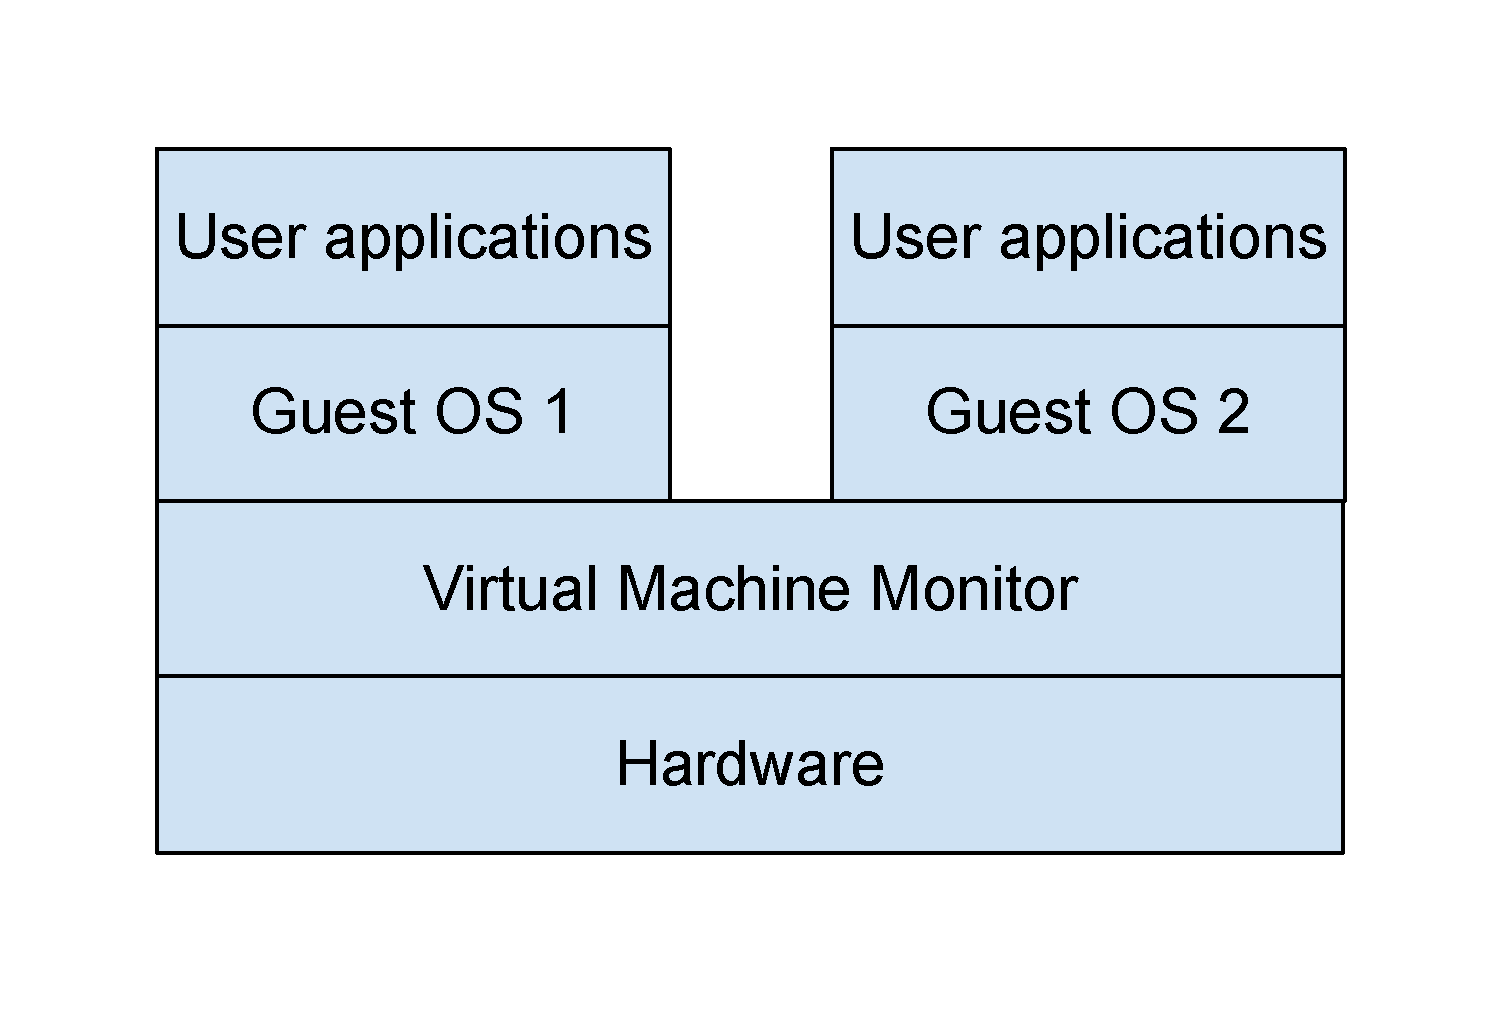
\includegraphics[scale = 1.0]{type-1-vmm.pdf}
\caption{An example of system using Type 1 VMMs.}
\label{fig:t1vmm}
\end{figure}

\begin{figure}[bt]
\centering
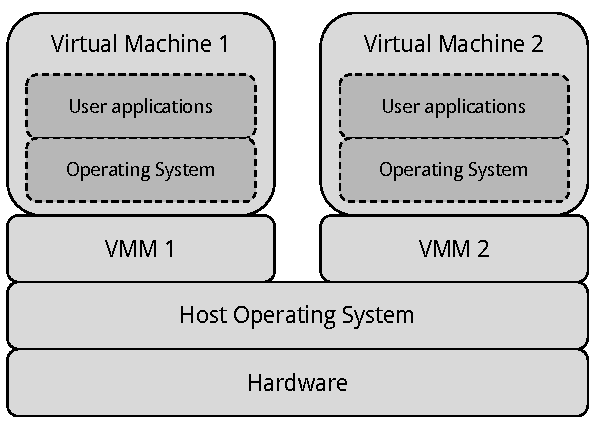
\includegraphics[scale = 1.0]{type-2-vmm.pdf}
\caption{An example of system using Type 1 VMMs.}
\label{fig:t2vmm}
\end{figure}



\vspace{0.5cm}

The different-ISA case is useful if you want to run legacy software on modern machines\footnote{Game console emulators are a common case 
of this kind of VM.} or if you want to test your software for compatibility with other architectures. In this case a VMM is basically a
full system emulator, capable to emulate the complete behaviour af a complex computer system.


\subsection{Process level Virtual Machines}
A very similar secondary classification applies also to process virtual machines, although at the ABI level. A VM can expose to the
application it executes (the guest application) the same ABI exposed to a regular process excecuting in the host system, or expose a 
completely different ABI.

Here the common case is when the ABI is different. The Java Virtual Machine is an example of this VM type: it executes code written 
conforming to an ABI (the Java bytecode) which is different by the ABI offered by the host OS. In this case the JVM engine is the VMM.
All interpreted language engines are VMs of this kind. Process VMs are also used for other purposes, such as runtime optimization
of binary code (see chapter 4 of \cite{ref:vmbook}), or binary translation in general.

\vspace{0.5cm}

The same-ABI case is just the concept of multiprogrammed OS, namely an OS capable of virtualize the CPU and
memory, offering to each process a \emph{virtual processor} and a \emph{virtual memory}. These two virtual resources make up
the enviroment (which provides some limited degree of isolation) where an OS process lives. We are so used to the multiprogramming
concept that we don't even think of it as being a form of virtualization. In this case the VMM is the OS itself (together with
the ISA which is designed to efficiently support multiprogramming).


\section{Virtual Machine Implementation}
\label{sec:vmimpl}

As showed in section \ref{sec:vmclass}, there are many types of conceptually different virtual machines.
Neverthless, all the VMs deal with executing code written for a certain environment (source code, or guest code),
using another environment (the host environment). This is a form \emph{emulation}: the term emulation refers to \emph{the process of
implementing the interface and functionality of a system on a system having a different interface and functionality}
(\cite{ref:vmbook} page 27).

The basic techniques employed to implement emulation are three: interpretation, dynamic translation, and hardware-based virtualization.
These techniques can be used alone or in combination to provide the virtual environment we want to implement.
Nowadays VMMs generally use a combination of the three methods.


\subsection{Interpretation}
The naive emulation technique is known as \emph{interpretation}.
Basically, the VMM has to do in software what a physical CPU would have done
in hardware. Take the current instruction (or statement, if we are dealing with high level languages VMs), excecute it updating the
VM status (which is an in-memory representation of all the VM resources, like registers, memories and the like), and go to the next
instruction. The VMM would then be implemented as a loop that, in each iteration, performs the fetch, decode and execute phases of
instruction execution.

\vspace{0.5cm}

Although writing an interpreter for a modern ISA or an interpreted programming languages can be a very long and complex process,
because of the complexity of the source language, the technique is conceptually easy. You just have to read an Instruction Set 
specification or a Programming Language specification and implement all the possible instructions/statement strictly respecting
the specified behaviour.

Being simple, this method is generally terribly inefficient if compared to the native execution of the source code on a processor
designed to execute the source ISA, because for each source instruction the VMM has to execute many host instructions (e.g. 30-100)
to perform in software all the necessary operations. In other words, the average \emph{translation ratio} is very high (e.g. 40).
On the other end, a big advantage is that the VMM has always the control over the execution of the source program, because it is 
executing the program step by step.

Many tricks can be implemented in order to improve the emulation performances. Some of these tecniques can be found in \cite{ref:vmbook}
(sections 2.1 through 2.4).


\subsection{Dynamic Translation}
A more sophisiticated form of emulation is called \emph{dynamic translation} or \emph{binary translation} or 
\emph{Just In Time compliation}, depending on the context.

Having to translate a source code in something else, an idea is to translate it into equivalent binary code that can be directly
executed on the host CPU. The VMM does this translation \emph{on the fly}, as soon as the source code is fetched from memory.
The method is intended to amortize the costs of interpretation, doing the repetitive work (fetch and decode) once or a few
times. 
The code execution step of a source instruction or a block of instructions, namely the translation, is generated once (or a few times)
and saved in a \emph{Code Cache}. The next time the source program flow goes through that block of source instructions, we don't have
to fetch, decode or translate, but just to execute the translation block.
The blocks of translated instructions can be connected directly to each other using native jump instructions, 
in the way suggested by the source program flow. After some time the code cache will become the complete translation of the source program
into the host ISA.

The final result is that the average translation ratio can be very close to 1 (e.g. less than 4), giving a nearly native performance,
or at least a performance that is acceptable also for performance sensitive applications.

\vspace{0.5cm}

The whole process is of course way more complicated than what has been presented here. Several problems are present, such as the 
\emph{code-discovery} problem that makes impossible to do a static translation, or the \emph{code-location} problems, that is due
to the different address space of the guest and host systems, or the state mapping problem, that is the way the VMM maps guest registers
and similar resources to the host ones.

Similarly to the interpretation method, with dynamic translation the VMM has (or can easily get) complete control over the guest code
execution: While doing the translation, it can put \emph{traps}\footnote{Point in the code that interrupts the guest
execution and give control to the VMM directly, or indirectly thorugh the host OS.} in the guest code wherever it wants.

For further informations on dynamic translation, see \cite{ref:vmbook} (sections 2.5 through 2.9).


\subsubsection{The same-ISA case}
\label{sec:sidt}
Interesting enough, interpretation and dynamic translation can make sense also in the same-ISA case. In this case the translation is
simplified, and most of the time the source code can execute natively on the host machine, without performance losses.

However there are some instructions that cannot be executed natively, because they access physical resources, because
are trying to access resources that do not exists on the physical machines, or because they are not easily virtualizable (see
\cite{ref:x86-virt} and section 8.2 of \cite{ref:vmbook}).

\vspace{0.5cm}

As a typical example, memory accesses addressing the I/O space or the memory mapped I/O can have side effects and then must be emulated 
in software. If the instruction was intended to access a physical resource that exists on the host, like a network adapter, the VMM 
cannot allow direct access to the device, because other processes or the host OS could be accessing the same device at the same time,
and certainly the host network driver and the guest network driver are not aware of each other.
If the instruction was intended to access a virtual network adapter (that doesn't exist on the host), the I/O instruction must be trapped
in order to emulate the device behaviour in software.


\subsection{Hardware-based virtualization}
\label{sec:hbv}
Due to the widespread use of VMs, the processor vendors have introduced processor extensions that allow for efficient and safe execution
of guest code in the same-ISA case. These hardware assists are intended to overcome some of the common problems arising when using
dynamic translation techniques, and at the same time they make it easy to execute guest code natively.
For the x86 ISA, both AMD and Intel have proposed their extensions, AMD-v (\cite{ref:amd-v}) and Intel VT-x (\cite{ref:intel-VT-x}).
These features provide all the means necessary to fully virtualize the x86 ISA. Since they fairly complex, we will only outline those
aspects that are intersting with respect to our work.

\vspace{0.5cm}

When the extension are present, the CPU is able to switch to a special mode, that we will call \emph{VM mode}, through a so called
\emph{VMEnter} instruction and switch back to normal mode through a so called \emph{VMExit} instruction.
When in VM mode, the CPU can execute guest code in a controlled environment. When necessary, the CPU can switch back to normal mode, 
starting to execute host code (VMM, OS or other processes).
The switch operation between the the host world and the guest world is conceptually similar to the more familiar process context switch,
since it includes saving the host (guest) state and loading the guest (host) state. These operation are done in hardware but are
still very expensive, expecially if we consider the additional software overhead involved in this host-guest transition, due to
OS operations and possible userspace/kernelspace transitions that could be necessary to transfer the control to the VMM or to the
guest.

The VM switches are necessary in some situations, such as dealing with I/O operations (see \ref{sec:sidt}), or when we want
to deliver an interrupt to the guest.

Since VM switches are very expensive, but sometimes necessary, trying to minimize them is fundamental if a VMM
wants to deliver good I/O performance.
